\documentclass[12pt,a4paper]{article}
\usepackage[top=1.5cm, bottom=1.5cm, left=2.0cm, right=1.5cm] {geometry}
\usepackage{amsmath,amssymb,txfonts}
\usepackage{tkz-euclide}
\usepackage{setspace}
\usepackage{lastpage}

\usepackage{tikz,tkz-tab}
%\usepackage[solcolor]{ex_test}
%\usepackage[dethi]{ex_test} % Chỉ hiển thị đề thi
\usepackage[loigiai]{ex_test} % Hiển thị lời giải
%\usepackage[color]{ex_test} % Khoanh các đáp án
\everymath{\displaystyle}

\def\colorEX{\color{purple}}
%\def\colorEX{}%Không tô màu đáp án đúng trong tùy chọn loigiai
\renewtheorem{ex}{\color{violet}Câu}
\renewcommand{\FalseEX}{\stepcounter{dapan}{{\bf \textcolor{blue}{\Alph{dapan}.}}}}
\renewcommand{\TrueEX}{\stepcounter{dapan}{{\bf \textcolor{blue}{\Alph{dapan}.}}}}

%---------- Khai báo viết tắt, in đáp án
\newcommand{\hoac}[1]{ %hệ hoặc
    \left[\begin{aligned}#1\end{aligned}\right.}
\newcommand{\heva}[1]{ %hệ và
    \left\{\begin{aligned}#1\end{aligned}\right.}

%Tiêu đề
\newcommand{\tenso}{iMath}
\newcommand{\tentruong}{Phần mềm Tạo đề ngẫu nhiên}
\newcommand{\tenkythi}{ĐỀ ÔN TẬP}
\newcommand{\tenmonthi}{Môn thi: Toán}
\newcommand{\thoigian}{}
\newcommand{\tieude}[1]{
   \begin{tabular}{cm{3cm}cm{3cm}cm{3cm}}
    {\bf \tenso} & & {\bf \tenkythi} \\
    {\bf \tentruong} & & {\bf \tenmonthi}\\
    && {\bf Thời gian: \bf \thoigian \, phút}\\
    && { \fbox{\bf Mã đề: #1}}
   \end{tabular}\\\\
    
   {Họ tên HS: \dotfill Số báo danh \dotfill}\\
}
\newcommand{\chantrang}[2]{\rfoot{Trang \thepage $-$ Mã đề #2}}
\pagestyle{fancy}
\fancyhf{}
\renewcommand{\headrulewidth}{0pt} 
\renewcommand{\footrulewidth}{0pt}
\usetikzlibrary{shapes.geometric,arrows,calc,intersections,angles,quotes,patterns,snakes,positioning}

\begin{document}
%Thiết lập giãn dọng 1.5cm 
%\setlength{\lineskip}{1.5em}
%Nội dung trắc nghiệm bắt đầu ở đây


\tieude{001}
\chantrang{\pageref{LastPage}}{001}
\setcounter{page}{1}
{\bf PHẦN I. Câu trắc nghiệm nhiều phương án lựa chọn.}
\setcounter{ex}{0}
\Opensolutionfile{ans}[ans/ans001-1]
\begin{ex}
 Cho hình chóp ${S.BCEF}$ có đáy là hình thoi tâm ${O}$. Gọi ${N,K}$ lần lượt là trung điểm của ${SB,SE}$. Khẳng định nào sau đây là khẳng định đúng? 
\begin{center}
 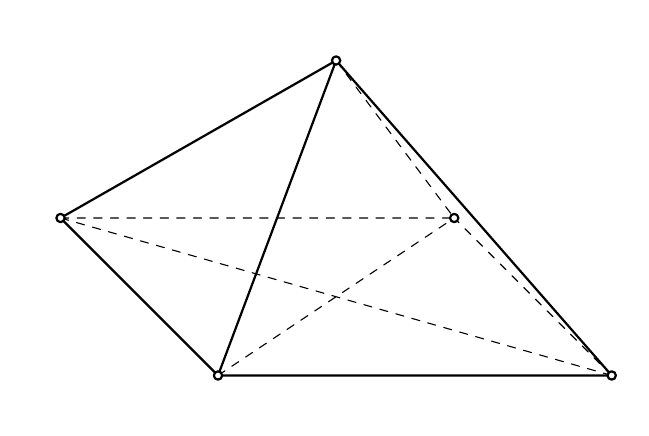
\begin{tikzpicture}[line join=round, line cap=round,thick]
\coordinate (B) at (0,0);
\coordinate (C) at (2,-2);
\coordinate (F) at (5,0);
\coordinate (E) at ($(C)+(F)-(B)$);
\coordinate (O) at ($(B)!0.5!(E)$);
\coordinate (S) at ($(O)+(0,3)$);
\draw(S)--(B) (S)--(C) (S)--(E) (B)--(C) (C)--(E);
\draw[dashed,thin](B)--(E) (B)--(F) (E)--(F) (S)--(F) (C)--(F);
\foreach \i/\g in {S/90,B/180,C/-90,E/-90,F/0}{\draw[fill=white](\i) circle (1.5pt) ($(\i)+(\g:3mm)$) node[scale=1]{};}
\end{tikzpicture}

\end{center}
\choice
{ $BE//(SCF)$ }
   { \True $NK//(BCE)$ }
     { $NK//(SBC)$ }
    { $CE//(ONK)$ }
\loigiai{\begin{center}
 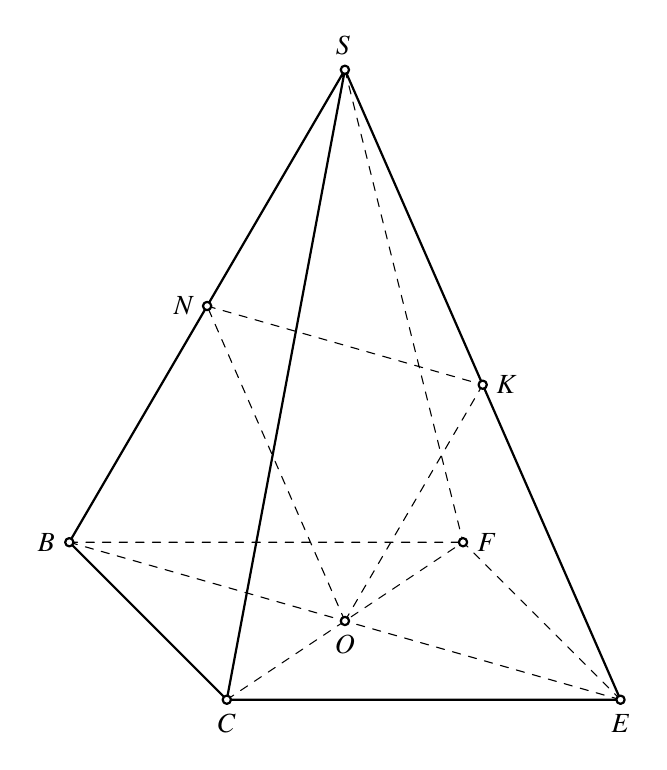
\begin{tikzpicture}[line join=round, line cap=round,thick]
		\coordinate (B) at (0,0);
		\coordinate (C) at (2,-2);
		\coordinate (F) at (5,0);
		\coordinate (E) at ($(C)+(F)-(B)$);
		\coordinate (O) at ($(B)!0.5!(E)$);
		\coordinate (S) at ($(O)+(0,7)$);
		\coordinate (N) at ($(B)!0.5!(S)$);
		\coordinate (K) at ($(E)!0.5!(S)$);
		\draw(S)--(B) (S)--(C) (S)--(E) (B)--(C) (C)--(E) ;
		\draw[dashed,thin](B)--(E) (B)--(F) (E)--(F) (S)--(F) (C)--(F) (O)--(N) (O)--(K) (N)--(K);
		\foreach \i/\g in {S/90,B/180,C/-90,E/-90,F/0,N/-180,K/0, O/-90}{\draw[fill=white](\i) circle (1.5pt) ($(\i)+(\g:3mm)$) node[scale=1]{$\i$};}
		\end{tikzpicture}

\end{center}
 
 $NK // BE \Rightarrow NK//(BCE)$. 
 }\end{ex}

\Closesolutionfile{ans}

 \begin{center}
-----HẾT-----
\end{center}

 %\newpage 
%\begin{center}
%{\bf BẢNG ĐÁP ÁN MÃ ĐỀ 1 }
%\end{center}
%{\bf Phần 1 }
% \inputansbox{6}{ans001-1}



\end{document}